\documentclass{report}

\usepackage{amsmath,amssymb}
\usepackage{graphicx}
\usepackage{enumitem}
\usepackage[total={6in,8in}]{geometry}
\usepackage{multicol}

\newcommand{\sol}{\textbf{Solution:}}
\newcommand{\proof}{\textbf{Proof:}}
\newcommand\perm[2][^n]{\prescript{#1\mkern-2.5mu}{}P_{#2}}
\newcommand\permtwo[2][^n]{{}_{#1}P_{#2}}
\newcommand\comb[2][^n]{{}_{#1}C_{#2}}
\newcommand\combtwo[2][^n]{\prescript{#1\mkern-2.5mu}{}C_{#2}}

\allowdisplaybreaks
\begin{document}
\begin{enumerate}[leftmargin=*]
    \item Diagram 1 shows the mapping of function $f$, such that $p$ is a constant.
          \begin{center}
              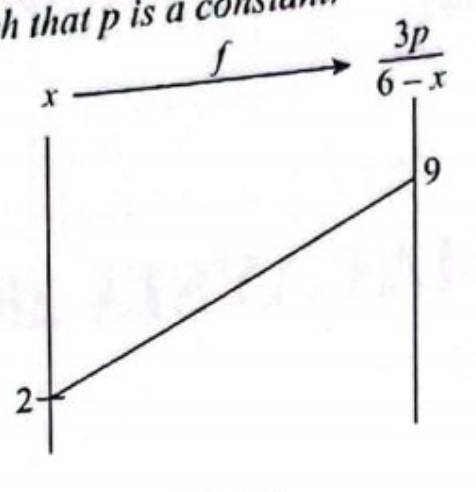
\includegraphics[width=0.3\textwidth]{./assets/p1.1.png}
          \end{center}
          \begin{enumerate}
              \item State the object which has no image.

                    \sol{}

                    The object which has no image when
                    \begin{align*}
                        6-x & =0 \\
                        x   & =6
                    \end{align*}

              \item Find the value of $p$. \sol{}
                    \begin{align*}
                        f(2)              & = 9  \\
                        \dfrac{3p}{6 - 2} & = 9  \\
                        \dfrac{3p}{4}     & = 9  \\
                        3p                & = 36 \\
                        p                 & = 12
                    \end{align*}
          \end{enumerate}

    \item \begin{enumerate}
              \item Express $p$ in terms of $k$ of
                    \begin{enumerate}
                        \item $x^{2 k+p}=1$,

                              \sol{}
                              \begin{align*}
                                  x^{2 k+p}  & =1        \\
                                  x^{2 k}x^p & =1        \\
                                  x^p        & =x^{-2 k} \\
                                  p          & =-2 k
                              \end{align*}

                        \item $a^p=(\sqrt[k]{a})^6$.

                              \sol{}
                              \begin{align*}
                                  a^p & =(\sqrt[k]{a})^6 \\
                                  a^p & =a^{\frac{6}{k}} \\
                                  p   & =\frac{6}{k}
                              \end{align*}
                    \end{enumerate}

              \item Given that $3+\dfrac{3^y}{3^{2(x+1)}}=84$, express $y$ in terms of $x$.

                    \sol{}
                    \begin{align*}
                        3+\dfrac{3^y}{3^{2(x+1)}} & =84       \\
                        \dfrac{3^y}{3^{2(x+1)}}   & =81       \\
                        3^{y-2(x+1)}              & =3^4      \\
                        y-2(x+1)                  & =4        \\
                        y                         & =4+2(x+1) \\
                        y                         & = 2x+6
                    \end{align*}
          \end{enumerate}

    \item \begin{enumerate}
              \item Derive that $\log _a m n=\log _a m+\log _a n$.

                    \sol{}

                    Let $\log _a m = p$ and $\log _a n = q$, $\log _a m n = r$.
                    \begin{align*}
                        a^p            & = m                   \\
                        a^q            & = n                   \\
                        a^r            & = m \times n          \\
                        a^p \times a^q & = a^{r}               \\
                        a^{p+q}        & = a^{r}               \\
                        p+q            & = r                   \\
                        \log _a m n    & = \log _a m+\log _a n
                    \end{align*}

              \item Hence, find the value of $u$ if $\log _u(u+3)+\log _u(u-1)=2$.

                    \sol{}
                    \begin{align*}
                        \log _u(u+3)+\log _u(u-1) & =2            \\
                        \log _u[(u+3)(u-1)]       & =2            \\
                        u^2+2u-3                  & =u^2          \\
                        2u-3                      & =0            \\
                        2u                        & =3            \\
                        u                         & =\dfrac{3}{2}
                    \end{align*}
          \end{enumerate}

          \newpage
    \item \begin{enumerate}
              \item Fei buys a block of ice cube. On the journey back home, the ice melts at the
                    rate of $5.5 \mathrm{~cm}^3$ per minute. Determine the rate of change of the
                    side length, in $\mathrm{cm} \text{s}^{-1}$, of the ice at the instant when the
                    side length is $15 \mathrm{~cm}$.

                    \sol{}
                    \begin{align*}
                        \dfrac{dV}{dt} & =-\dfrac{5.5}{60}                                    \\
                                       & = -\dfrac{11}{120} \mathrm{~cm}^3 \mathrm{~s}^{-1}   \\
                        V              & = s^3                                                \\
                        \dfrac{dV}{ds} & = 3s^2                                               \\
                        \dfrac{ds}{dt} & = \dfrac{ds}{dV} \times \dfrac{dV}{dt}               \\
                                       & = \dfrac{1}{\dfrac{dV}{ds}} \times \dfrac{dV}{dt}    \\
                                       & = \dfrac{1}{3s^2} \times -\dfrac{11}{120}            \\
                                       & = -\dfrac{11}{360 s^2} \mathrm{~cm} \mathrm{~s}^{-1} \\
                    \end{align*}
                    When $s=15$,
                    \begin{align*}
                        \dfrac{ds}{dt} & = -\dfrac{11}{360 \times 15^2}                     \\
                                       & = -\dfrac{11}{81000} \mathrm{~cm} \mathrm{~s}^{-1}
                    \end{align*}

              \item Given that $\dfrac{d}{d x}\left[\dfrac{5}{1-x^2}\right]=g(x)$, find
                    $\displaystyle\int[2 g(x)+3] d x$.

                    \sol{}
                    \begin{align*}
                        \int[2 g(x)+3] d x & = 2 \int g(x) d x+3 \int d x      \\
                                           & = 2\times \dfrac{5}{1-x^2}+3x + C \\
                                           & = \dfrac{10}{1-x^2}+3x + C
                    \end{align*}
          \end{enumerate}

    \item The coordinates of points $P$ and $Q$ are $(2,3)$ and $(q, 2 q)$ respectively.
          Given that $\overrightarrow{P Q}$ is a unit vector. Using the vectors's
          triangle law, find the possible values of $q$.

          \sol{}
          \begin{align*}
              \overrightarrow{PQ} & = \overrightarrow{P O}+\overrightarrow{OQ} \\
                                  & = \overrightarrow{OQ}-\overrightarrow{OP}  \\
                                  & = q\vec{i}+2q\vec{j}-2\vec{i}-3\vec{j}     \\
                                  & = (q-2)\vec{i}+(2q-3)\vec{j}               \\
              \text{Magnitude}    & = \sqrt{(q-2)^2+(2q-3)^2}                  \\
                                  & = 1                                        \\
              (q-2)^2+(2q-3)^2    & = 1                                        \\
              q^2-4q+4+4q^2-12q+9 & = 1                                        \\
              5q^2-16q+13         & = 1                                        \\
              5q^2-16q+12         & = 0                                        \\
              (5q-6)(q-2)         & = 0                                        \\
              q                   & = \dfrac{6}{5}, 2
          \end{align*}

    \item The variables $x$ and $y$ are related by the equation $y=\dfrac{p x}{q x-1}$,
          such that $p$ and $q$ are constants. If $a$ graph of $y$ against $x$ is drawn,
          its curve will pass through $\left(\dfrac{1}{2},-6\right)$ whereas a straight
          line with the gradient of $\dfrac{1}{8}$ is obtained when a graph of
          $\dfrac{1}{y}$ against $\dfrac{1}{x}$ is drawn.

          Find the value of $p$ and of $q$.

          \sol{}

          When $x=\dfrac{1}{2}$, $y=-6$,
          \begin{align*}
              -6           & =\dfrac{p \times \dfrac{1}{2}}{q \times \dfrac{1}{2}-1} \\
              -6           & =\dfrac{\dfrac{p}{2}}{\dfrac{q}{2}-1}                   \\
              -6           & =\dfrac{p}{q-2}                                         \\
              p            & =-6q+12                                                 \\
              y            & =\dfrac{p x}{q x-1}                                     \\
              \dfrac{1}{y} & = \dfrac{q x-1}{p x}                                    \\
                           & = -\dfrac{1}{p}\dfrac{1}{x} + \dfrac{q}{p}              \\
              \dfrac{1}{8} & = -\dfrac{1}{p}                                         \\
              p            & = -8                                                    \\
              -8           & = -6q+12                                                \\
              -6q          & = -20                                                   \\
              q            & = \dfrac{10}{3}
          \end{align*}

    \item Diagram 2 shows sectors $A O B$ and COD inscribed in a circle with centre $O$.
          \begin{center}
              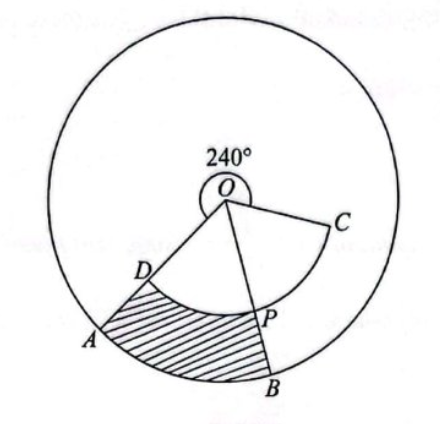
\includegraphics[width=0.4\textwidth]{./assets/p1.7.png}
          \end{center}
          The radius of the circle and the radius of the sector $C O D$ is $h \mathrm{~cm}$ and $k \mathrm{~cm}$ respectively. The lengths of arc $C P$ and arc $P D$ are equal. It is given that the perimeter of the minor sector $A O B$ is $15.235 \mathrm{~cm}$ and the area of the shaded region is $8.376 \mathrm{~cm}^2$.

              [Use $\pi=3.142$]
          \begin{enumerate}
              \item State the $\angle C O D$, in terms of $\pi$,

                    \sol{}
                    \begin{align*}
                        \angle C O D & = 360^\circ - 240^\circ \\
                                     & = 120^\circ
                    \end{align*}

              \item Hence, calculate the value of $h$ and of $k$ to the nearest integer.

                    \sol{}
                    \begin{align*}
                        \angle DOP                      & = \angle POC = \dfrac{120}{2} = 60^\circ = \dfrac{\pi}{3} \text{ radian} \\
                        \text{Perimeter of sector } AOB & = 2\pi h + 2k = 15.235 \text{ cm}                                        \\
                    \end{align*}
          \end{enumerate}

    \item \begin{enumerate}
              \item Diagram 3 shows the standard normal distribution graph.
                    \begin{center}
                        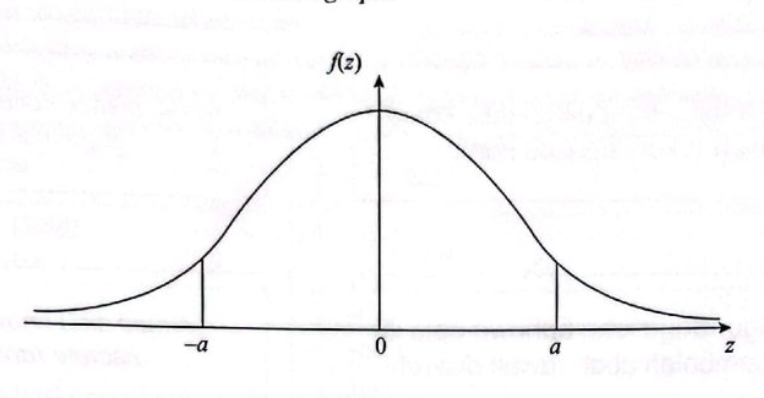
\includegraphics[width=0.4\textwidth]{./assets/p1.8a.png}
                    \end{center}
                    On Diagram 3, shade the region(s) to represent $P(|Z| \geq a)$.

              \item Diagram 4 shows the standard normal distribution graph which is divided into
                    three equal parts.
                    \begin{center}
                        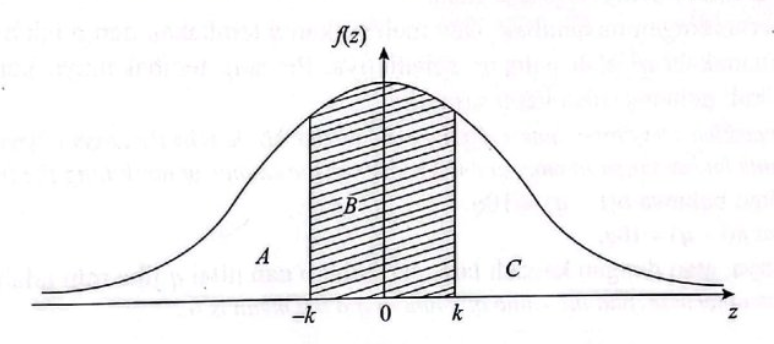
\includegraphics[width=0.4\textwidth]{./assets/p1.8b.png}
                    \end{center}
                    State
                    \begin{enumerate}
                        \item the value of $k$,
                        \item the mode for part $A$.
                    \end{enumerate}
          \end{enumerate}

    \item \begin{enumerate}
              \item Diagram 5 shows the conversation between Nash and Cikgu Wong.
                    \begin{center}
                        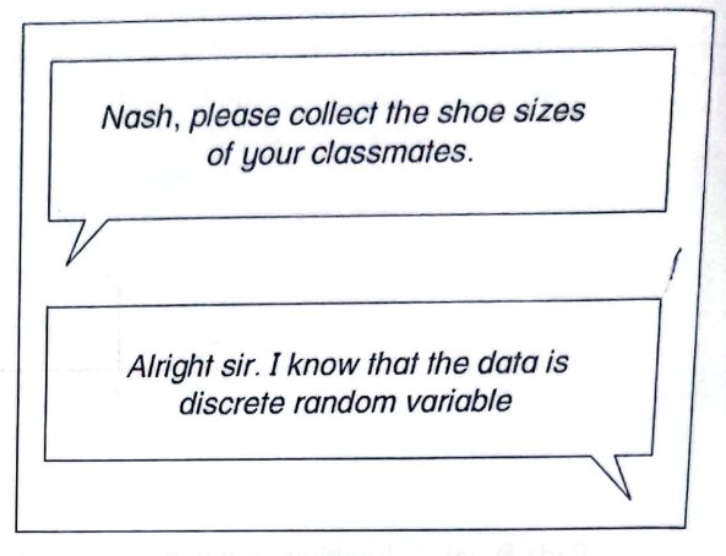
\includegraphics[width=0.4\textwidth]{./assets/p1.9a.png}
                    \end{center}
                    Is Nash's statement true? Give your justification.

              \item In a shooting competition, Dev fires $n$ shots and $p$ is the chance that his
                    shots hit the target whereas $q$ is the otherwise chance. The chance of his
                    shots hit the target at most one is 11 times of the chance of not hitting the
                    target.
                    \begin{enumerate}
                        \item Show that $n(1-q)=10 q$.
                        \item Hence, or otherwise, find the value of $p$ and of $q$ if the mean is 6.
                    \end{enumerate}
          \end{enumerate}

    \item \begin{enumerate}
              \item A school bookstore is having a stock clearance promotion which involves 8
                    different pens and 10 different notebooks. Ani will spend RM24 in the
                    promotion. Table 1 shows the prices for a unit of each item.
                    \begin{center}
                        \begin{tabular}{|c|c|c|}
                            \hline Item               & Pen  & \begin{tabular}{c}
                                                                   Notebook
                                                               \end{tabular} \\
                            \hline \begin{tabular}{c}
                                       Price (RM)
                                   \end{tabular} & 2.00 & 4.00                   \\
                            \hline
                        \end{tabular}
                    \end{center}
                    Find the number of different ways Anvi can buy the item if
                    \begin{enumerate}
                        \item she wants to buy notebooks only,
                        \item the number of notebooks is at most equal to the number of pens.
                    \end{enumerate}

              \item Diagram 6 shows an example of five-character password formed by using letters
                    and digits on a computer screen.
                    \begin{center}
                        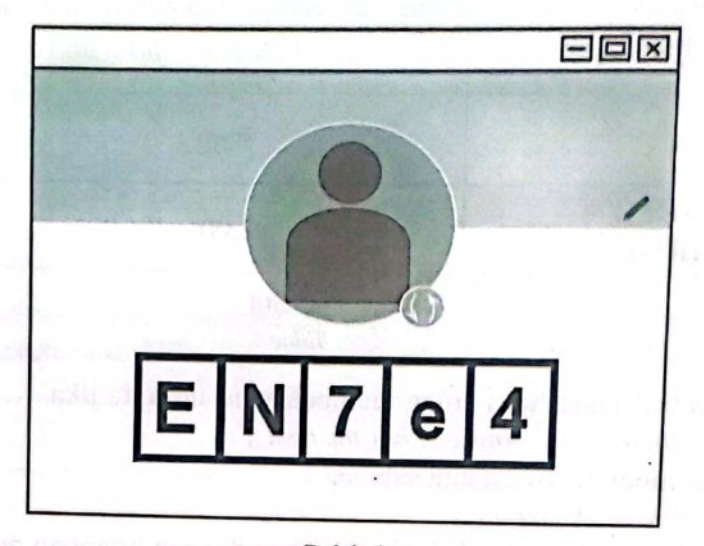
\includegraphics[width=0.4\textwidth]{./assets/p1.10b.png}
                    \end{center}
                    Find the number of different passwords if
                    \begin{center}
                        (i) the first three characters are A8a without repetition,
                        (ii) the first character must be a non-vowel capital letter and followed by at least two prime numbers placed adjacently.
                    \end{center}
          \end{enumerate}

    \item Diagram 7 shows triangle $A B C$.
          \begin{center}
              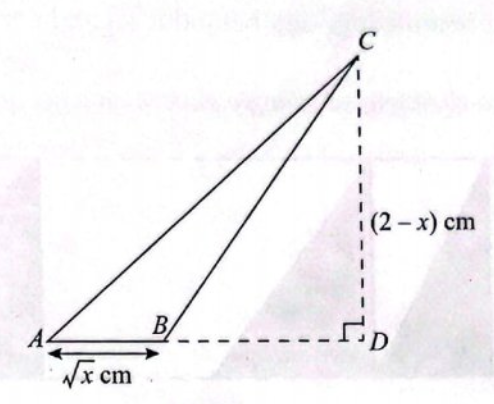
\includegraphics[width=0.4\textwidth]{./assets/p1.11.png}
          \end{center}
          It is given that $B C=(2+x) \mathrm{cm}, A D^2=1+\sqrt{2}$ and $A B D$ is a straight line. Show that $x=\dfrac{1+5 \sqrt{2}}{49} \mathrm{~cm}$.

    \item Diagram 8 shows a purple coloured right angled triangle pattern on a net of a
          rectangular roll of paper.
          \begin{center}
              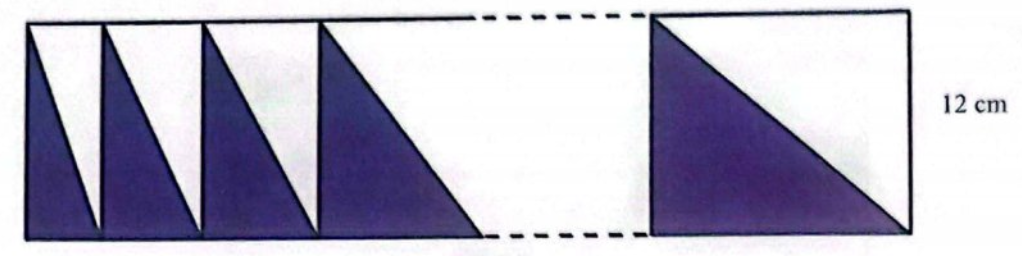
\includegraphics[width=0.7\textwidth]{./assets/p1.12.png}
          \end{center}
          It is given that the length of the base of the first triangle is a $\mathrm{cm}$ and the length of each subsequent base increases by $d \mathrm{~cm}$.
          \begin{enumerate}
              \item Derive that the length of the base of the $n^{\text {th }}$ triangle is
                    $T_n=a+(n-1) d$.
              \item On the net, the $31^{\text {st }}$ purple coloured triangle is the last
                    triangle with an area of $72 \mathrm{~cm}^2$ and it is given that $a=30
                        \mathrm{~d}$.
                    \begin{enumerate}
                        \item Find the value of $d$, in $\mathrm{cm}$.
                        \item Zul wants to send a number of rolls of the paper to his friend through a
                              courier company. Table 2 shows an information related to parcel delivery
                              charges.
                              \begin{center}
                                  \begin{tabular}{|c|c|c|}
                                      \hline \begin{tabular}{c}
                                                 Mass
                                             \end{tabular} & $0-2.5 \mathrm{~kg}$ & \begin{tabular}{c}
                                                                                        Every subsequent $500 \mathrm{~g}$
                                                                                    \end{tabular} \\
                                      \hline \begin{tabular}{c}
                                                 Rate (RM)
                                             \end{tabular} & 9.00                 & 1.20                                         \\
                                      \hline
                                  \end{tabular}
                              \end{center}

                              If Zul has RM15 and the mass of the paper per $\mathrm{cm}^2$ is $4 \times
                                  10^{-5} \mathrm{~kg}$, calculate the maximum number of rolls of the paper that
                              can be sent.
                    \end{enumerate}
          \end{enumerate}

    \item \begin{enumerate}
              \item Diagram 9 shows angle $\theta$ on a Cartesian plane.
                    \begin{center}
                        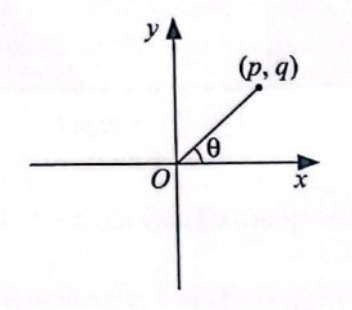
\includegraphics[width=0.33\textwidth]{./assets/p1.13a.png}
                    \end{center}
                    \begin{enumerate}
                        \item On Diagram 9, label the position of $-\theta$.
                        \item State the value of $\tan (-\theta)$ in terms of $p$ and $q$.
                    \end{enumerate}

              \item Solve the equation $2 \cos x=\sqrt{3} \cot x$ for $0^{\circ} \leqslant x
                        \leqslant 360^{\circ}$.

              \item It is given that $\tan m=p$, such that $m$ is a reflex angle. Express $\cos
                        \left(\dfrac{\pi}{3}-m\right)$ in terms of p.
          \end{enumerate}

    \item Diagram 10 shows a curve of a quadratic function $f(x) = 2x^2 + hx - 2k + 5$,
          such that $h$ and $k$ are constants. The curve has a minimum point at $T$.
          \begin{center}
              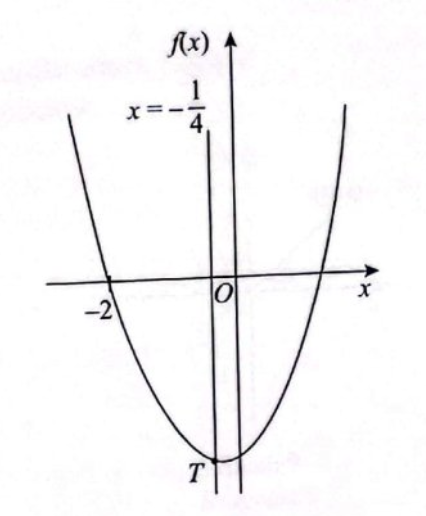
\includegraphics[width=0.4\textwidth]{./assets/p1.14.png}
          \end{center}
          \begin{enumerate}
              \item Determine the range of values of $x$ of $f(x)>0$.
              \item Prove that $k>\dfrac{40-h^2}{16}$. item Using the method of completing the
                    square, find the minimum value of function $f(x)$ in terms of $k$.
          \end{enumerate}

    \item \begin{enumerate}
              \item Diagram 11 shows a line segment $AC$.
                    \begin{center}
                        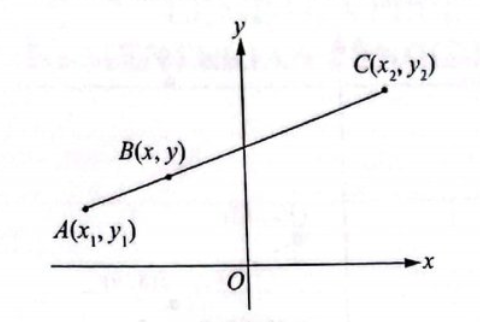
\includegraphics[width=0.5\textwidth]{./assets/p1.15a.png}
                    \end{center}
                    It is given that point $B$ divides the line segment $A C$ in the ratio of $m: n$. Show that $y=\dfrac{n y_1+m y_2}{m+n}$.

              \item It is given that $P(x, y)$ moves such that its distance from
                    $R\left(\frac{3}{2},-\frac{1}{2}\right)$ is 2.5 times its distance from the
                    $y$-axis. Find the equation of locus of $P$.
          \end{enumerate}
\end{enumerate}
\end{document}